\documentclass[14pt]{article}
\usepackage{amsmath}
\usepackage{amssymb}
\usepackage{cancel}
\usepackage{graphicx}
\usepackage{geometry}
\usepackage{tikz}
\usetikzlibrary{automata, positioning, arrows}
\geometry{
	a4paper,
	total={170mm,257mm},
	left=20mm,
	top=17mm,
}
\tikzset{
	->, % makes the edges directed
	>=stealth, % makes the arrow heads bold
	node distance=2cm, % specifies the minimum distance between two nodes. Change if necessary.
	every state/.style={thick, fill=gray!15}, % sets the properties for each ’state’ node
	initial text=$\text{start}$, % sets the text that appears on the start arrow
}
\begin{document}
	\title{Finite State Machines}
	\author{Saptarshi Dey}
	\maketitle
	\section{Questions on Deterministic Finite State Automata}
	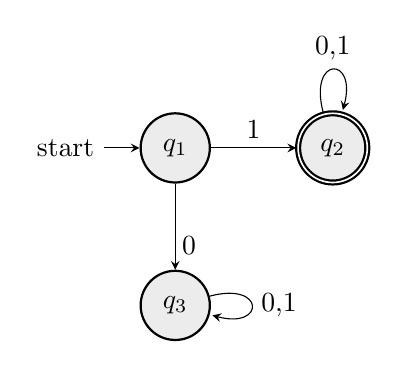
\begin{tikzpicture}
			\node[state, initial] (q1) {$q_1$};
			\node[state, accepting, right of=q1] (q2) {$q_2$};
			\node[state, below of=q1] (q3) {$q_3$};
	\draw 	(q1) edge[above] node{1} (q2)
			(q1) edge[below] node{$\ \ \ 0$} (q3)
			(q2) edge[loop above] node{0,1} (q2)
			(q3) edge[loop right] node{0,1} (q3);
	\end{tikzpicture}
	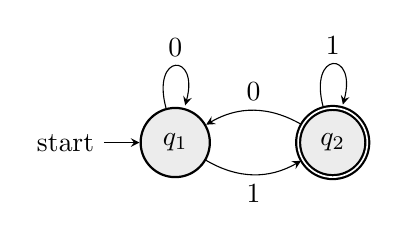
\begin{tikzpicture}
			\node[state, initial] (q1) {$q_1$};
			\node[state, accepting, right of=q1] (q2) {$q_2$};
	\draw 	(q1) edge[loop above] node{0} (q1)
			(q1) edge[below,bend right] node{1} (q2)
			(q2) edge[loop above] node{1} (q2)
			(q2) edge[above,bend right] node{0} (q1);
	\end{tikzpicture}
	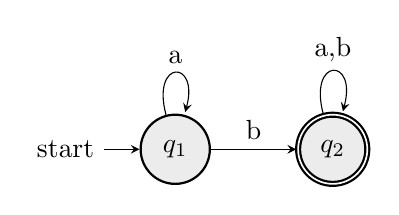
\begin{tikzpicture}
			\node[state, initial] (q1) {$q_1$};
			\node[state, accepting, right of=q1] (q2) {$q_2$};
	\draw 	(q1) edge[loop above] node{a} (q1)
			(q1) edge[above] node{b} (q2)
			(q2) edge[loop above] node{a,b} (q2);
	\end{tikzpicture}
	\\
	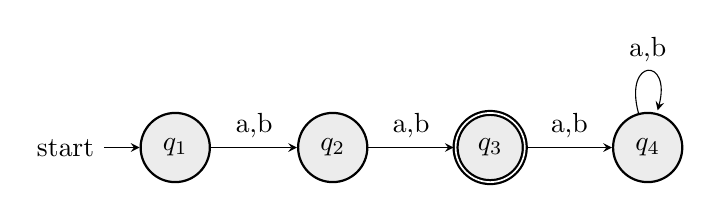
\begin{tikzpicture}
			\node[state, initial] (q1) {$q_1$};
			\node[state, right of=q1] (q2) {$q_2$};
			\node[state, accepting, right of=q2] (q3) {$q_3$};
			\node[state, right of=q3] (q4) {$q_4$};
	\draw	(q1) edge[above] node{a,b} (q2)
			(q2) edge[above] node{a,b} (q3)
			(q3) edge[above] node{a,b} (q4)
			(q4) edge[loop above] node{a,b} (q4);
	\end{tikzpicture}
	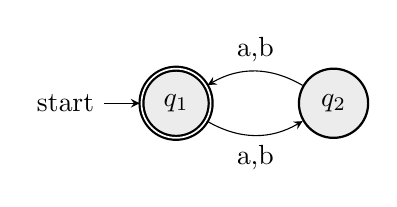
\begin{tikzpicture}
			\node[state, accepting, initial] (q1) {$q_1$};
			\node[state, right of=q1] (q2) {$q_2$};
	\draw 	(q1) edge[below,bend right] node{a,b} (q2)
			(q2) edge[above,bend right] node{a,b} (q1);
	\end{tikzpicture}
	\\ \\
	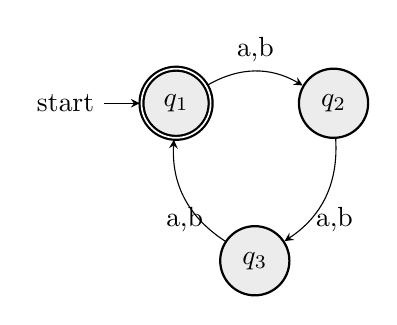
\begin{tikzpicture}
			\node[state, accepting, initial] (q1) {$q_1$};
			\node[state, right of=q1] (q2) {$q_2$};
			\node[state] at (1, -2) (q3) {$q_3$};
	\draw 	(q1) edge[above,bend left] node{a,b} (q2)
			(q2) edge[below,bend left] node{$ \ \ \text{a,b}$} (q3)
			(q3) edge[below,bend left] node{a,b} (q1);
	\end{tikzpicture}
	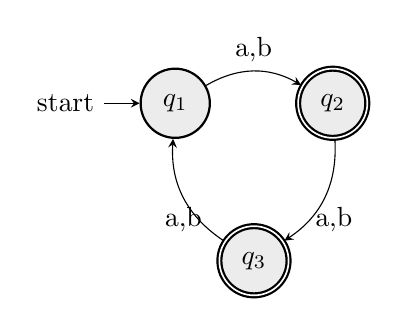
\begin{tikzpicture}
			\node[state, initial] (q1) {$q_1$};
			\node[state, accepting, right of=q1] (q2) {$q_2$};
			\node[state, accepting,] at (1, -2) (q3) {$q_3$};
	\draw 	(q1) edge[above,bend left] node{a,b} (q2)
			(q2) edge[below,bend left] node{$ \ \ \text{a,b}$} (q3)
			(q3) edge[below,bend left] node{a,b} (q1);
	\end{tikzpicture}
	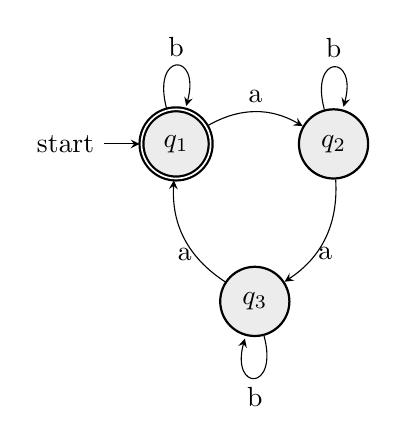
\begin{tikzpicture}
			\node[state, accepting, initial] (q1) {$q_1$};
			\node[state, right of=q1] (q2) {$q_2$};
			\node[state] at (1, -2) (q3) {$q_3$};
	\draw 	(q1) edge[above,bend left] node{a} (q2)
			(q1) edge[loop above] node{b} (q1)
			(q2) edge[below,bend left] node{a} (q3)
			(q2) edge[loop above] node{b} (q2)
			(q3) edge[below,bend left] node{a} (q1)
			(q3) edge[loop below] node{b} (q3);
	\end{tikzpicture}
	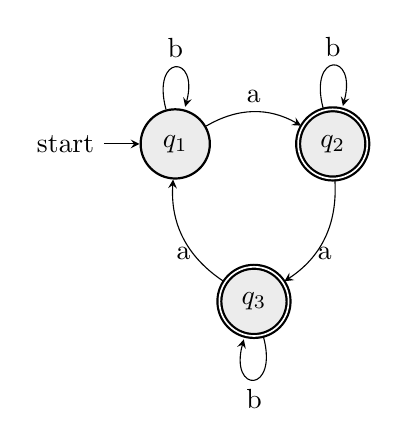
\begin{tikzpicture}
			\node[state, initial] (q1) {$q_1$};
			\node[state, accepting, right of=q1] (q2) {$q_2$};
			\node[state, accepting,] at (1, -2) (q3) {$q_3$};
	\draw 	(q1) edge[above,bend left] node{a} (q2)
			(q1) edge[loop above] node{b} (q1)
			(q2) edge[below,bend left] node{a} (q3)
			(q2) edge[loop above] node{b} (q2)
			(q3) edge[below,bend left] node{a} (q1)
			(q3) edge[loop below] node{b} (q3);
	\end{tikzpicture} 
	\\
	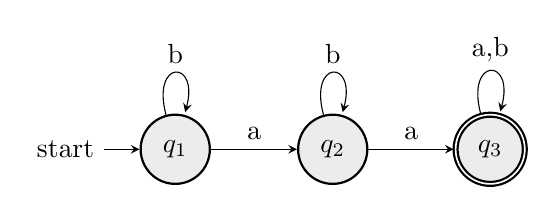
\begin{tikzpicture}
			\node[state, initial] (q1) {$q_1$};
			\node[state, right of=q1] (q2) {$q_2$};
			\node[state, accepting, right of=q2] (q3) {$q_3$};
	\draw 	(q1) edge[above] node{a} (q2)
			(q2) edge[above] node{a} (q3)
			(q1) edge[loop above] node{b} (q1)
			(q2) edge[loop above] node{b} (q2)
			(q3) edge[loop above] node{a,b} (q3);
	\end{tikzpicture}
	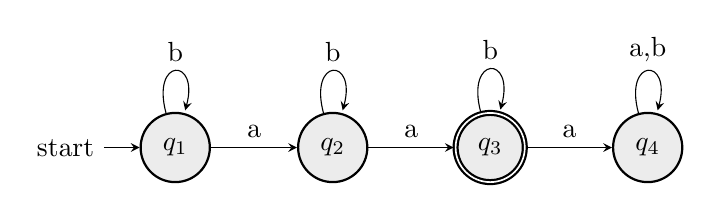
\begin{tikzpicture}
			\node[state, initial] (q1) {$q_1$};
			\node[state, right of=q1] (q2) {$q_2$};
			\node[state, accepting, right of=q2] (q3) {$q_3$};
			\node[state, right of=q3] (q4) {$q_4$};
	\draw 	(q1) edge[above] node{a} (q2)
			(q2) edge[above] node{a} (q3)
			(q3) edge[above] node{a} (q4)
			(q1) edge[loop above] node{b} (q1)
			(q2) edge[loop above] node{b} (q2)
			(q3) edge[loop above] node{b} (q3)
			(q4) edge[loop above] node{a,b} (q4);
	\end{tikzpicture}
	\\
	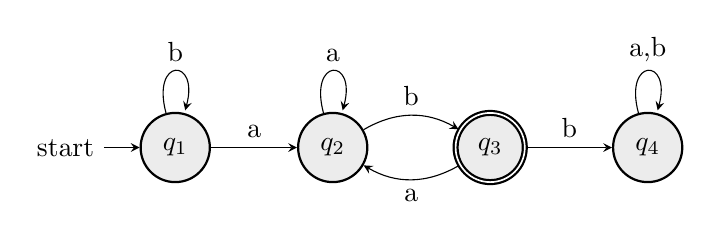
\begin{tikzpicture}
			\node[state, initial] (q1) {$q_1$};
			\node[state, right of=q1] (q2) {$q_2$};
			\node[state, accepting, right of=q2] (q3) {$q_3$};
			\node[state, right of=q3] (q4) {$q_4$};
	\draw 	(q1) edge[above] node{a} (q2)
			(q2) edge[above, bend left] node{b} (q3)
			(q3) edge[above] node{b} (q4)
			(q1) edge[loop above] node{b} (q1)
			(q2) edge[loop above] node{a} (q2)
			(q3) edge[below, bend left] node{a} (q2)
			(q4) edge[loop above] node{a,b} (q4);
	\end{tikzpicture}
\end{document}